\chapter{Eigenes Verfahren}\label{chp:EigVerfahren}
Diese Arbeit besteht aus drei gro�e Hauptschritte, n�mlich Hintergrundsubtraktion, Sch�tzung der K�rperhalterung mit Histogrammanalyse und Erkennung au�ergew�hnlicher Situation mit Fuzzylogik  

\section{Hintergrundsubtraktion}\label{chp:BackgroundSubtraction}
\subsection{Vergleichen verschiedener Methoden}
In dieser Masterarbeit ist Hintergrundsubtraktion ein wichtiger Baustein. Ein gro�es Problem ist wie ein korrekter Hintergrund erstellt werden kann, damit man sich bewegtes Objekt robust erkennen kann. F�r diese Arbeit wurden verschiedenen moderne Methoden (Gaussian Mixture Model, Kern Density Estimation und Vibe) ausprobiert und verglichen. Die alle genannte Methoden wurden schon in ~\ref{sec:Grundlage1} theoretisch beschrieben. In diesem Abschnitt geht es um Bewertungen von Hintergrundsubtraktionsverfahren. Bei \acs{GMM} wird eine Mischung von 5-Gau�schen Verteilung modelliert und eine Anzahl von 100 letzte Frames wird als "History"\ angewendet. Mit dem Lernrate $0.01$ funktioniert das \acs{GMM} Verfahren gut in unserem Test. F�r das \acs{AGMM} nehmen wir auch die gleichen Parameters, um den Vergleich der Hintergrundsubtraktionsverfahren objektiv zu bewerten. Bei \acs{KDE} handelt es sich um eine Berechnung von Intensit�tswerte f�r einen Pixel, deshalb wird nur ein Parameter von 100 als "History" wie bei \acs{AGMM} in diesem Fall eingesetzt. Wie in \cite{barnich2009vibe} schon gemeint, Vibe ist ein nicht-parametrisches Verfahren und weshalb kein Parameter wird hier gebraucht. 

\begin{figure}[htpb]
	\centering
	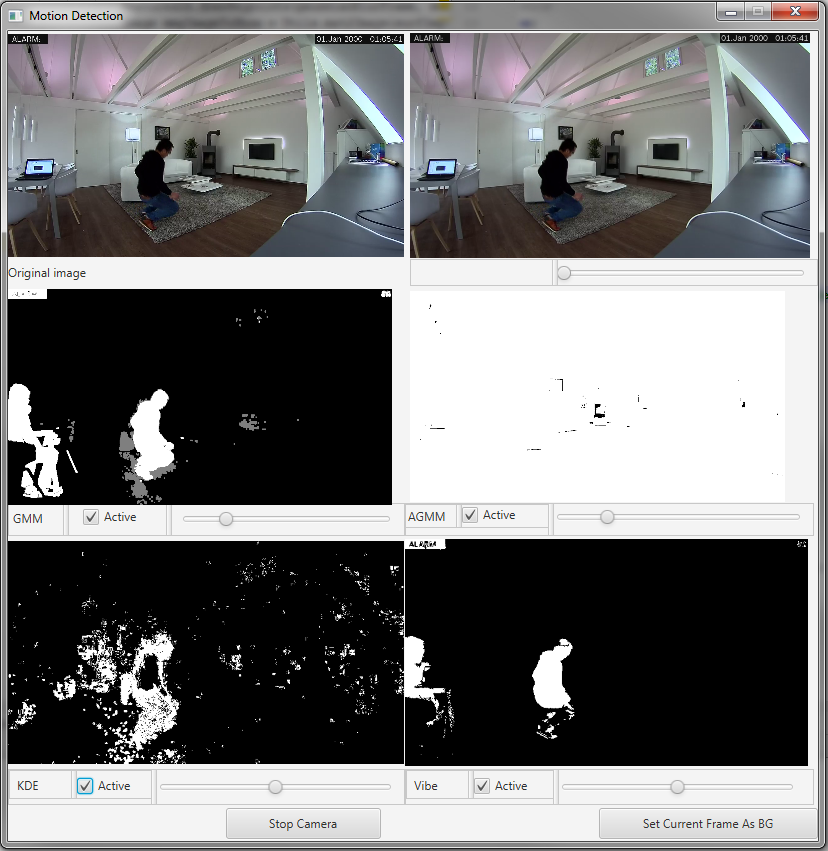
\includegraphics[width=1\textwidth]{fig/motiondetrection.png}
	\caption{Vergleichen von verschiedene Techniken an Hintergrundsubtraktion (a) Weichzeichnen (b) GMM (c) AGMM. (d) KDE (e) Vibe} 
	\label{fig:compare_bgsubtraction}
\end{figure}
Aus dieser Grafik \ref{fig:compare_bgsubtraction} wird deutlich, dass AGMM und Vibe ziemlich besser als die zweit andere. Hier ist kritisch anzumerken, dass Vibe und KDE l�ngere Verarbeitungszeit als den Rest brauchen. Das erste Ziel der Arbeit ist die Untersuchung der Hintergrundsubtraktion, damit eine beste Silhouette erkannt werden kann. Anhand des Schaubildes kann man erkennen, dass AGMM ein guter Kandidat f�r Hintergrundsubtraktion ist. Viele Videos in verschieden Orte mit verschiedene K�rperhaltung wurden f�r diese Arbeit aufgenommen, damit die Qualit�t der Software gut gepr�ft wird.  Anhand der Abbildung \ref{fig:compare_bgsubtraction} und Verarbeitungszeit wird deutlich, dass AGMM vern�nftige Methode f�r unser Ziel und deswegen wird AGMM f�r diese Arbeit entschieden.\\
Die oben genannte Hintergrundsubtraktionsverfahren basieren auf die �nderung des Intensit�tswerten von jedem Pixel, deshalb liefern die Verfahren ein Schwarzwei�bild mit viel Rausch zur�ck. Um die Rausch zu entfernen, wird Erosion und Dilatation zum Einsatz gebracht, die zwei Verfahren sind zwei grundlegende Operationen bei der morphologischen Bildverarbeitung, auf der alle anderen morphologischen Operationen basieren. Unter Erosion kann man verstehen ein Verfahren, das ein Bild mit einer einfachen, vordefinierten Form untersucht und daraus Schlussfolgerungen zieht, wie diese Form in die Formen im Bild verfehlt. Und Dilatation ist ein umgekehrtes Verfahren von Erosion, es versucht ein Bild zu erweitern mit passender Form von originalem Bild. Eingaben f�r die zwei Verfahren sind ein originales Bild $A$ und einen Filter $B$. Wenn das strukturierende Element $B$ ein Zentrum hat, kann die Erosion von A durch B als der Ort von Punkten verstanden werden, die durch das Zentrum von B erreicht werden, wenn B sich in A bewegt. Angenommen, dass der Ursprung $B$ in seiner Mitte ist, �berlagert f�r jedes Pixel in $A$ der Ursprung von $B$, wenn $B$ vollst�ndig in $A$ enthalten ist, wird das Pixel bei Erosion beibehalten, ansonsten gel�scht. Aber bei Dilatation �berlagert jeder Pixel in $A$ der Ursprung von $B$ und der Pixel wird in der Erweiterung von $A$ und $B$ enthalten. Um die zwei Operationen besser zu verstehen, wurden zwei Beispiele f�r Erosion und Dilatation in Abbildungen \ref{fig:erosion} und \ref{fig:dilatation} dargestellt.
\begin{figure}[htpb]
	\centering
	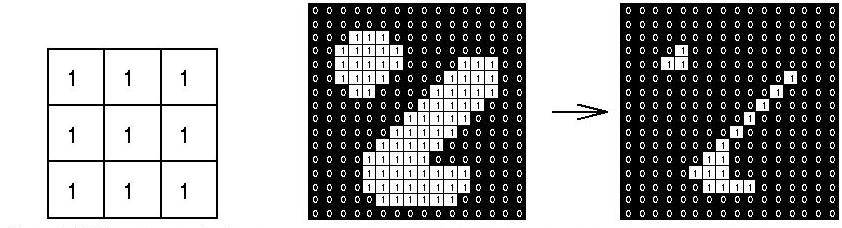
\includegraphics[width=1\textwidth]{fig/erosion.jpg}
	\caption{Erosion} 
	\label{fig:erosion}
\end{figure}
\begin{figure}[htpb]
	\centering
	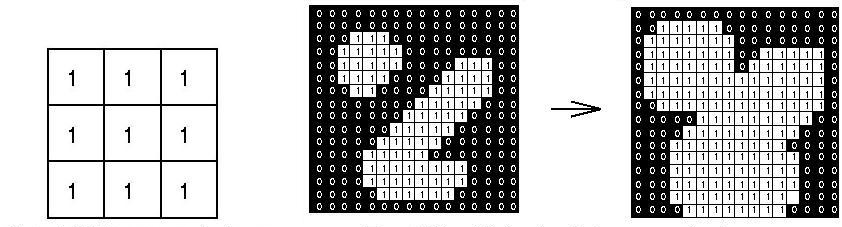
\includegraphics[width=1\textwidth]{fig/dilatation.jpg}
	\caption{Dilatation} 
	\label{fig:dilatation}
\end{figure}

Erosion wird in diesem Fall angewendet, um Rausch nach dem Hintergrundsubtraktion zu entfernen. Es folgt auch eine kleine �nderung an der Silhouette. Um die genannte �nderung zu vermeiden wird Dilatation hier genutzt. Die Abbildung \ref{fig:eroanddila} zeigt, dass nach Erosion unerwartete Rausch au�er Silhouette entfernt ist und auch die Silhouette leicht gesch�digt ist. Aber nach der Dilatation wird die Silhouette besser vervollst�ndigt. 

\begin{figure}[htpb]
	\centering
	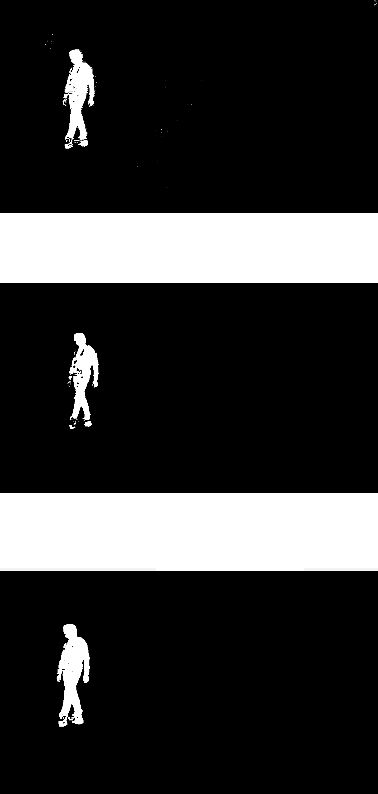
\includegraphics[width=0.65\textwidth]{fig/eroanddila.png}
	\caption{Ergebnis nach Erosion und Dilatation} 
	\label{fig:eroanddila}
\end{figure}

\subsection{Eine Verbesserung f�r Hintergrundsubtraktion}
Im Allgemein wird jeder Pixel von aktuellem Bild erst berechnet, ob er zu Hintergrund oder Vordergrund geh�rt, und dann wird den Pixel wieder nach jedem Frame in Hintergrundmodell hinzugef�gt. Das bedeutet, wenn ein Mensch sich bewegt von $A$ nach $B$ und auf $B$ so lang zum Stillstand kommt, wird der Mensch wieder in Hintergrund zugeordnet. Und das Problem muss unbedingt gel�st werden, weil die Arbeit um Erkennung einer au�ergew�hnlichen Situation geht, indem ein Unfall passieren kann und Person kann wahrscheinlich auf dem Boden lang liegen. Das Problem liegt an Aktualisierung des Hintergrundmodells, deshalb wird eine Methode in diese Stelle erstellt, um das Problem zu vermeiden. Das erste Frame wird als eine Hintergrundbild in Schwarzwei� abgelagert. Der Unterschied zwischen aktuellem Bild in Schwarzwei� und dem abgelagerten Hintergrundbild wird pixelweise gerechnet.



\subsection{Ergebnisse der eigene Hintergrundsubtraktion}
\section{Sch�tzung der K�rperhalterung mit Histogrammanalyse}
Im Abschnitt \ref{chp:BackgroundSubtraction} 
\section{Erkennung au�ergew�hnlicher Situation}